\documentclass[12pt,a4paper]{article}
  \usepackage[utf8]{inputenc}
  \usepackage[brazil]{babel}
  \usepackage{graphicx}
  \usepackage{color}
  \usepackage{hyperref}
  \usepackage{abnt-alf}
  \usepackage[top=3cm,bottom=2cm,left=3cm,right=2cm]{geometry}
  \usepackage{indentfirst}
  
  \begin{document}
  
  % CAPA
  \pagestyle{empty}
  \begin{center}
  \large  \textbf{UNIVERSIDADE PRESBITERIANA MACKENZIE}
  \large  \textbf{PROGRAMA DE PÓS-GRADUAÇÃO EM}\\
  \large  \textbf{ENGENHARIA ELÉTRICA E COMPUTAÇÃO}\\
  \vskip 2.0cm
  \textbf{\large Fernando Cainelli Tolentino}\\
  \vskip 4.0cm
  \setlength{\baselineskip}{1.5\baselineskip}
  \textbf{\large Latent Dirichlet Allocation: Visualizando e Explorando Documentos}\\
  \vskip 4.5cm
  \end{center}
  \hfill{\vbox{\hsize=8.5cm\noindent\strut
  Projeto de Pesquisa apresentado ao Programa\break
  de Pós-Graduação em Engenharia Elétrica e\break
  Computação da Universidade Presbiteriana\break
  Mackenzie como parte dos requisitos para a\break
  aprovação na disciplina de Metodologia do\break
  Trabalho Científico.}\\
  \strut}
  \vskip 3.0cm
  \textbf{\normalsize Orientador: Prof. Dr. Leandro Augusto da Silva}\\
  \vskip 2.0cm
  \begin{center}
  São Paulo\\
  2017\\
  \end{center}
  
  % RESUMO
  \newpage
  \thispagestyle{plain}
  \pagenumbering{roman}
  \begin{center}
  \large
  \textbf{RESUMO}
  \end{center}
  \renewcommand{\baselinestretch}{0.6666666}
  O resumo deve apresentar, em no máximo 250 palavras, o tema da pesquisa, os objetivos, o recorte teórico-metodológico e os resultados almejados. A proposta do projeto de pesquisa é estabelecer uma primeira delimitação do trabalho que será realizado ao longo do Mestrado. Neste sentido, a apresentação do projeto de pesquisa é realizada por meio de um texto que possui a estrutura de divisões deste documento, a formatação de um mínimo de dezessete (17) a vinte (20) laudas de conteúdo em papel A4 branco com espaçamento entre linhas de 1,5.
  \\[0.5cm]
  \begin{flushleft}
  {\bf Palavras-chave:} {\it apresentação, separada por vírgulas, de três a seis unitermos significativos para o trabalho.}
  \end{flushleft}
  
  % SUMÁRIO
  \newpage
  \thispagestyle{empty}
  \tableofcontents
  
  % DESENVOLVIMENTO
  \newpage
  \pagestyle{plain}
  \pagenumbering{arabic}
  \renewcommand{\baselinestretch}{1.5}
  \normalsize
  \section{INTRODUÇÃO}
  Ao longo da introdução deve-se desenvolver o tema de forma a construir um cenário que possibilite compreender a delimitação do estudo e o contexto onde este se encontra inserido.
  
  Neste item também é necessário apresentar o objetivo geral da pesquisa, ou seja, a meta proposta para a investigação. De forma complementar, os objetivos específicos, também presentes na introdução, constituem os elementos de trabalho que permitem alcançar o objetivo geral. Como os objetivos traduzem ações que serão executadas ao longo da pesquisa, a apresentação destes no texto requer a utilização de verbos no infinitivo.
  
  Ainda, deve-se colocar a hipótese: uma afirmação provisória que será confirmada ou refutada pelo pesquisador ao longo da investigação.
  
  Finalmente, é preciso descrever as partes do projeto de pesquisa.
  
  \section{JUSTIFICATIVA}
  Com acúmulo cada vez mais crescente de informações digitalizadas e armazenadas na forma de: artigos, blogs, jornais, e-mails, livros, mensagens instantâneas, redes sociais, entre outros, a tarefa de organizar, indexar e buscar essas informações é fundamental. Para possibilitar usuários navegar por esses documentos e encontrar a informação desejada, utilizamos hoje dois métodos principais, links e busca. Links correlatam trechos de um documento a outro, são muito úteis pois possibilitam uma extensão da leitura e aprofundamento do conhecimento, direcionando o leitor a termos ou assuntos relacionados de alguma forma ao documento original. Apesar de ser uma ótima maneira de fornecer conteúdo diretamente relacionado, encontramos desafios na aplicação em escala, pois muitas vezes, essa ferramenta  é implementada de forma manual pelo o autor. A busca por outro lado, requer um processo que pode ser automatizado de forma efetiva, pois indexando as informações presentes nos documentos, permite ao usuário procurar um documento por palavra chave ou metadados presentes. Esse processo é muito disseminado, e motores de busca utilizam de técnicas sofisticadas em diversas áreas como ranqueamento de resultados e similaridade de palavras para melhorar essa experiência. O trabalho de Mikolov, T. et al. (2013) por exemplo, possibilita em escala, fornecer funcionalidades como sugestões de termos de pesquisa baseado na ordem das palavras digitadas além de extensão de busca utilizando termos similares.
  
  Essas técnicas são poderosas para interagirmos com nossos documentos, no entanto há uma lacuna, imagine explorar documentos por meio de temas de interesse específico, visualizar as palavras mais relevantes em cada tema e explorar os documentos com a usabilidade de um mapa, com possibilidade de zoom in, zoom out, além de visualizar a relação entre documentos de uma maneira intuitiva, por proximidade. Essa, pode ser uma forma complementar de busca aos métodos citados no parágrafo anterior. A aplicação desse método pode ser em qualquer corpus, no entanto, como exemplo, vamos demonstrar como aplicação em um corpus contendo documentos de e-mail.
  E-mails possuem informações que podem aprimorar ainda mais a experiência de exploração, pois os documentos podem ser exibidos em forma de nós, conectando remetentes a destinatários e aprimorando ainda mais a exibição dos resultados da pesquisa.
  
  Pesquisas apontam que em 2017 atingiremos uma média de 269 bilhões de e-mails enviados e recebidos diariamente, e é esperado continuar a crescer a uma taxa média de 4.4\% ao ano nos próximos quatro anos, atingindo 319.6 bilhões ao final de 2021 (The Radicati Group, Inc., 2017).
  
  \begin{table}[h]
    \centering
    \caption{Tráfego de Email Mundial Diário  (Bi). The Radicati Group, Inc. Email Statistics Report, 2017-2021, p. 3. (2017)}
    \begin{tabular}{l*{6}{c}r}
    &					2017 &	2018 &	2019 &	2020 &	2021 & \\
    \hline
    Quantidade de E-mails &			269.0 &	281.1 &	293.6 &	306.4 &	319.6 & \\
    Crescimento(\%) &  	&		4.5\% &	4.4\% &	4.4\% &	4.3\% & \\
    \hline
    \end{tabular}
  \end{table}
  
  A taxa de crescimento da quantidade de mensagens enviadas e recebidas impressiona, não só por se tratar de uma técnologia dos anos 70, mas principalmente pela forte adoção de novos recursos de comunicação como: mensagem instantânea, redes sociais, videoconferência, chat, etc. A comunicação via e-mail permanece sólida principalmente em empresas, estas, por sua vez, tem a necessidade de aplicar a inteligência nos negócios para manter-se competitivas. O Business Intelligence deve ser utilizado não só em escopos diretamente relacionados ao negócio, como clientes, produtos, etc. mas também nos indiretos, como colaboradores para se obter insights, melhoria dos processos e otimização. Frequentemente, e-mails são deixados fora da equação pela falta de ferramentas específicas e complexidade para tratar de dados não estruturados, neste artigo, queremos promover um método complementar de exploração de documentos, para isso, vamos utilizar um conjunto de documentos de e-mail de uma empresa e fazer uso do modelo generativo probabilístico proposto por Blei et al.(2003), Latent Dirichlet Allocation, além de técnicas de processamento e visualização de conhecimento. Faremos uso das mesmas técnicas, na análise exploratória do conjunto de dados, espera-se também obter informações relevantes que possam ser utilizadas na compreensão no negócio da empresa.
  
  
  \section{REFERENCIAL TEÓRICO}
  
  
  % Abaixo encontram-se exemplos de citação:
  
  % Citação entre parênteses após paráfrase \cite{andrade99}.
  
  % Citação em que o autor \citeonline{gil91} é referenciado durante a explicação.
  
  No campo de processamento de linguagem natural e recuperação de informação, existem diversas técnicas de agrupamento, análise e extração de sentido de um conjunto de dados de textos. Nesta seção, vamos apresentar as técnicas disponíveis e trabalhos relatos relevantes utilizados neste artigo.
  
  \subsection{K-MEANS}
  
  O algoritmo K-Means, assinala a cada objeto de um conjunto de dados à um grupo, foi introduzido inicialmente por J. MacQueen(1967) e é um dos algoritmos mais estudados na literatura. O algoritmo é inicializado com dois parâmetros principais, o número de clusters, ou grupos, disponíveis para os objetos no dataset serem classificados e um vetor de objetos que representa o conjunto de dados. Cada objeto no conjunto de dados pode ser assinalado à um grupo a cada iteração. Primeiro determinamos os centróides iniciais, centróides são a representação de um grupo e seu valor é dado pela média dos objetos desse grupo, são iniciados randomicamente, como proposto  pelo trabalho original, ou utilizando algum algoritmo de otimização, em alguns casos, o K-Means pode convergir para grupos distintos dependendo do valor inicial dos centróides. Existem diversos estudos que adotam diferentes algoritmos e técnicas para inicialização dos centróides, Yuan F. et al.(2004) propuseram um método  para se obter os centróides iniciais de acordo com a distribuição do conjunto de dados, em sua pesquisa obtiveram melhor acurácia com essa técnica quando comparada a inicialização randômica proposta no trabalho original de J. MacQueen(1967).
  
  O próximo passo é rodar o algoritmo até que convirja. Para cada iteração, o algoritmo assinala cada objeto ao grupo cujo centróide está mais próximo e calcula a nova média do grupo para então ajustar os valores dos centróides. Para determinar a distância entre um objeto observado e os centróides, K-Means utiliza a distância Euclidiana que calcula a diferença entre um objeto vetor \(X=(x1, x2... x_n)\)e um centróide vetor \(C=(c1, c2... c_n)\) com a seguinte fórmula: 
  
  \begin{equation}
  d(X\,C) = \sqrt{(x_1 - c_1)^2 + (x_2 - c_2)^2 ... + (x_n - c_n)^2}
  \end{equation}
  
  O objeto $X$ será assinalado ao grupo cujo centróide tem a menor distância Euclidiana. Em seguida, o algoritmo percorre cada grupo calculando a média dos objetos nele presente, e define esse valor ao centróide do grupo. O processo se repete até que os objetos não troquem de grupo.
  
  O algoritmo K-Means assinala cada objeto do conjunto de dados a exatamente um grupo, no entanto, para problemas que objetos podem pertencer a mais de um grupo, ou quando grupos de dados são representados por uma forma não circular, uma vez que é  utilizada a distância Euclidiana para assinalar objetos a grupos, um modelo misto, ou mixture model, podem obter agrupamentos com melhores representações.
  
  \subsection{LATENT DIRICHLET ALLOCATION}
  
  Latent Dirichlet Allocation, ou LDA, é um modelo generativo probabilístico proposto por Blei et. al. (2003), esse modelo é usado em diversas áreas como análise de sentimento, classificação de documentos, bioinformática, agrupamento de dados entre outros. LDA sugere que palavras carregam uma forte informação semântica, e que documentos com assuntos similares contém também um grupo de palavras similares. Os tópicos latentes, ou ocultos, são portanto descobertos identificando o grupo de palavras no corpus que co-ocorrem frequentemente dentro dos documentos. A idéia básica do LDA é:
  
  \begin{enumerate}
    \item Cada documento é representado por uma mescla de tópicos.
    \item Cada tópico é formado por uma distribuição de palavras.
  \end{enumerate}
  
  LDA encontra o modelo probabilístico de um conjunto de dados. Enquanto modelos como os de Mistura de Unigramas, assumem que cada documento exibe características de apenas um tópico, o modelo do LDA  permite que documentos contenham múltiplos tópicos ao mesmo tempo e com relevância distintas. Nesta seção, vamos discorrer sobre as principais características do trabalho original de Blei. A pesquisa de D.J. Hu(2009) foi complementar durante essa seção para melhor compreender o trabalho original.
  
  Antes de nos aprofundarmos na descrição do algoritmo, façamos uma introdução da terminologia formal e notações usada nesta seção.
  
  \begin{enumerate}
    \item Uma $palavra$ é a mais básica unidade de dado, definida com um item de um vocabulário indexado por \(w \in \{1,. . . , V\}\)  , onde $V$ é o número de palavras únicas dentro de um corpus, também denominado vocabulário. Palavras são representadas como um vetor de base unitária.
    \item Um documento é uma sequência de $N$ palavras denotadas por \(\textbf{ w} = (w_1, w_2,. . . ,  w_N)\).
    \item Um corpus é uma coleção de $M$ documentos denotados por \(\textbf{ D} = \{\textbf{ w}_1, \textbf{ w}_2, . . ., \textbf{ w}_M\}\).
  \end{enumerate}
  
  \subsection{PROCESSO GENERATIVO}
  O LDA assume que documentos são criados via um processo generativo no qual palavras nos documentos são geradas. Dado o tamanho do documento, nós escolhamos uma mistura de tópicos usando a distribuição multinomial de tópicos para escolher as palavras que devem ser usada para preencher a cota de cada tópico. ex: Temos um grupo de artigos que assumimos que tais artigos podem ser classificados em quatro tópicos, Esportes, Animais, Tecnologia e Artes, cada tópico pode ser definido pela seguinte lista de palavras:
  
  \begin{itemize}
    \item \textbf{ Esportes:} bola, futebol, basquete, gol, pontos, corrida, natação.
    \item \textbf{ Animais:} coelho, cachorro, gato, galinha, touro, aranha.
    \item \textbf{ Tecnologia:} computadores, smartphone, tablet, tech, câmera, web.
    \item \textbf{ Artes:} cinema, dança, música, canção, pintura, cores, movimento, instrumento.
  \end{itemize}
  
  Com as informações apresentadas acima, queremos gerar um novo artigo que contenha 75\% artes e 25\% esporte, primeiro determinamos o tamanho do artigo em número de palavras, então para cada tópico escolhido para mistura, selecionamos as palavras de cada tópico proporcionalmente a ele. O LDA usa esse conceito de forma reversa para determinar a distribuição de tópicos por documento e a distribuição de palavras por um tópico. O processo generativo permite diferentes graus de relevância de uma palavra em um tópico, e um tópico em um documento, na teoria da probabilidade isso é chamado permutabilidade, ou exchangeability(Aldous, 1985). O processo generativo pode ser descrito formalmente como:
  
  Para cada documento indexado por $d \in \{1,. . . , M\}$ em um corpus $D$:
  
  \begin{enumerate}
    \item Escolha um vetor de tópico $\theta _d$ de dimensão $K$ da distribuição $p(\theta|\alpha)=Dirichlet(\alpha)$.
    \item Para cada uma das $N$ palavras($w_n$) dentro de um documento:
    \begin{enumerate}
      \item Escolha um tópico \(z_n \in \{1,. . . , K\}\) do Multinomio($\theta$).
      \item Da distribuição de probabilidade multinomial \(p(w_n=1| z_n=j,\beta)=\beta _{ij}\)  desenhe uma palavra $w_n$ dado tópico $z_n$.
    \end{enumerate}
  \end{enumerate}
  
  O  hiperparâmetro $\alpha$ é um vetor de dimensão $K$ com items \(\alpha _i>0\) e é uma distribuição Dirichlet priori da distribuição de tópicos por documento, o hiperparâmetro $\beta$ é uma distribuição Dirichlet priori da distribuição de palavras por tópicos. $\theta _d$ é a distribuição de tópicos para o documento $d$. $Z_{dn}$ e $W_{dn}$ são as variáveis a nível de palavras e são amostradas uma vez para cada palavra em cada documento.
  
  Uma variável de distribuição Dirichlet randômica $\theta$ com dimensão $K$ tem como propriedade: $\theta ^i \geq 0, \displaystyle\sum_{i=1}^{K} \theta ^i = 1$ e têm a seguinte densidade probabilística:
  
  \begin{equation}
  p(\theta|\alpha) = \frac{\Gamma(\displaystyle\sum_{i=1}^{K} \alpha _i)}{\displaystyle\prod_{i=1}^{K} \Gamma(\alpha _i)} \theta _1 ^{\alpha _i - 1} ...  \theta _K ^{\alpha _K - 1}
  \end{equation}
  
  A distribuição Dirichlet é utilizada pois possui um conjunto de propriedades importantes que possibilitam um processo de inferência e estimação de parâmetros mais simples. A distribuição é da família exponencial, conjuga com a distribuição multinomial, possui dimensões finitas e possui estatística suficiente. A distribuição  acima dá a cada documento seu próprio vetor de distribuição que indica a relevância de cada tópico $K$ para com aquele documento. O processo generativo acima define a distribuição conjunta para cada documento $\textbf{ w}_d$.
  
  A distribuição conjunta de uma mistura de tópico $\theta$, um conjunto de $K$ tópicos $z$, e um conjunto de $N$ palavras $w$, dado os hiperparâmetros $\alpha$ e $\beta$ é dado por:
  
  
  \begin{equation}
  p(\theta,\textbf{z},\textbf{w}|\alpha,\beta) = p(\theta|\alpha) \prod_{n=1}^{N} p(z_n|\theta)p(w_n|z_n,\beta)
  \end{equation}
  
  
  A Figura 1 ilustra o Plate Notation do modelo LDA, as caixas são pratos representando réplicas, o $M$ denota o número de documentos que é associado ao prato externo e o interno representa as palavras dentro de um documento, onde $N$ denota o número de palavras.
  
  \begin{figure}[h]
    \centering
      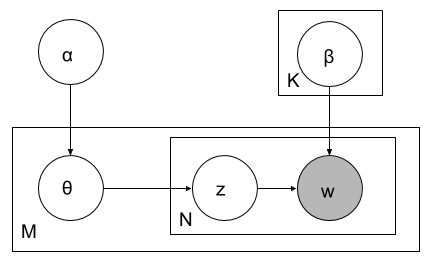
\includegraphics[height=10cm]{images/figure_1.png}
      \caption{Plate Notation representando o modelo LDA, adaptado de Blei et al. Latent Dirichlet Allocation. Journal of Machine Learning Research, 2003.(p. 1003)}
  \end{figure}
  
  onde $p(z_n | \theta)$é simplesmente $\theta _i$ para cada $i$ único, tal que $z_{ni}=1$. Nós obtemos a distribuição marginal de um documento $d$ integrando sobre $\theta$ e somando sobre $z$.
  
  \begin{equation}
  p(\textbf{w}|\alpha,\beta)=\int{p(\theta|\alpha)\Bigg(\prod_{n=1}^{N}\sum_{z_n} p(z_n|\theta)p(w_n|z_n,\beta)\Bigg)d\theta}
  \end{equation}
  
  A probabilidade de um corpus é obtida com o produto das probabilidades marginais de um documento:
  
  \begin{equation}
  p(D|\alpha,\beta)= \prod_{d=1}^{M} \int{p(\theta _d|\alpha)\Bigg(\prod_{n=1}^{N_d}\sum_{z_{dn}} p(z_{dn}|\theta _d)p(w_{dn}|z_{dn},\beta)\Bigg)d\theta _d}
  \end{equation}
  
  \subsection{INFERÊNCIA}
  
  A Eq.(3) foi baseada nos hiperparâmetros antecedentes $\alpha$ e $\beta$, nesta seção, nós descrevemos o procedimento para inferência.
  
  O problema de inferência principal a se resolver é o de se computar a distribuição posteriori das distribuições latentes:
  
  \begin{equation}
  p(\theta,\textbf{z}|\textbf{w},\alpha,\beta) = \frac{p(\theta,\textbf{z},\textbf{w}|\alpha,\beta)}{p(\textbf{w}|\alpha,\beta)}
  \end{equation}
  
  A distribuição acima é intratável de se computar em geral, o numerador é a distribuição conjunta das variáveis randômicas, que são computáveis para qualquer configuração de variáveis ocultas, o denominador é a distribuição marginal, em teoria, pode ser calculada somando a distribuição conjunta de todas instâncias possíveis, no entanto, o número de estruturas de tópicos é exponencialmente grande, e essa soma é intratável de se computar (Blei, 2012). Para normalizar a distribuição da Eq.(4) é utilizado a distribuição marginal, de todos os documentos em um corpus:
  
  \begin{equation}
  p(\textbf{w}|\alpha,\beta)=\frac{\Gamma(\sum_{i}\alpha_i)}{\prod_{i}\Gamma(\alpha_i)}\int{\Bigg(\prod_{i=1}^{k}\theta_i^{\alpha_i-1}\Bigg)} \Bigg(\prod_{n=1}^{N}\sum_{i=1}^{K}\prod_{j=1}^{V}(\theta_i\beta_{ij})^{w_n^j}\Bigg)d\theta
  \end{equation}
  
  Embora a distribuição posterior é intratável devido ao acoplamento do $\theta$ and $\beta$, existe uma variedade de algoritmos de aproximação de inferência que podem ser usados, os métodos comumente encontrados na literatura são baseados em amostragem ou variação.
  
  O algoritmo de amostragem mais comum para modelação de tópicos é o Gibbs Sampling, uma instanciação especial da Cadeia de Markov Monte Carlo (MCMC) (Jordan, et al. 1999), uma sequência de variáveis randômicas, uma dependente da anterior. O algoritmo roda coletando amostras da distribuição assintótica e então aproximando a distribuição com as amostras coletadas. O problema reside em não saber ao certo  quando o algoritmo convergiu para solução, além dos seus requisitos de memória, já que escala linearmente com o número de palavras em um corpus, isso torna o algoritmo não adotável em uma conjunto de dados muito grande(Řehůřek, 2011).
  
  O método mais utilizado em modelos de variável latente é o algoritmo variacional Expectation-Maximization(EM), que permite a estimação de parâmetros não supervisionada de maneira computacionalmente eficiente, o método determinístico de aproximação EM resulta em uma estimativa tendenciosa. Em cada iteração é atualizado os parâmetros computando os valores esperados das variáveis sobre a distribuição posterior na Eq.(7).
  
  
  \begin{figure}[h]
    \centering
      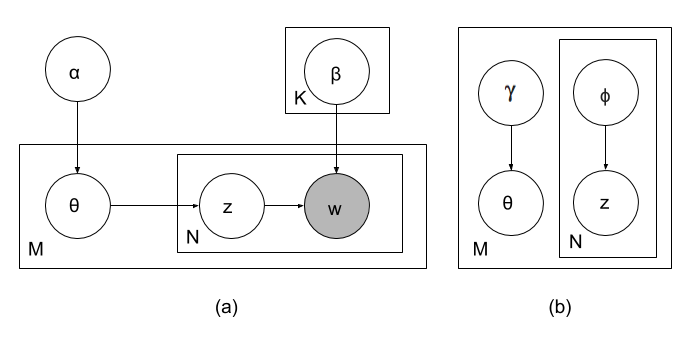
\includegraphics[height=10cm]{images/figure_2.png}
      \caption{(a) Representação gráfica do modelo LDA. (b) A aproximação variacional para a distribuição posteriori. Adaptado de Blei et al. Latent Dirichlet Allocation. Journal of Machine Learning Research, 2003.(p. 1003)}
  \end{figure}
  
  A idéia de Blei de utilizar inferência variacional baseada na convexidade é de se fazer o uso da desigualdade de Jensen para obter um limite inferior ajustável na verossimilhança(Jordan et al., 1999) onde os parâmetros variacionais são escolhidos através de um processo de otimização, tentando encontrar o limite inferior mais próximo em cada iteração. Considerando a Figura 2(a), a problemática do acoplamento dos parâmetros $\theta$ e $\beta$ surge devido às bordas entre $\theta$, $z$, e nó $w$, removendo-os, também estamos removendo as dependências entre as variáveis que tornam a equação intratável. Com isso, acabamos com um Plate Notation simplificado com parâmetros variacionais livres ilustrados na Figura 2(b), obtendo a família de distribuição de probabilidade nas variáveis ocultas, que é caracterizada pela seguinte distribuição variacional:
  
  \begin{equation}
  q(\theta,\textbf{z}|\gamma,\phi)=q(\theta|\gamma)\prod_{n=1}^{N}q(z_n|\phi_n)
  \end{equation}
  
  \section{METODOLOGIA}
  % Descrição detalhada e sequencial dos procedimentos científicos (métodos e técnicas) estabelecidos para atingir os objetivos propostos inicialmente para a pesquisa.
  
  \section{CRONOGRAMA}
  % O cronograma do projeto de pesquisa deverá apresentar as etapas do trabalho e a previsão do tempo necessário para a realização de cada uma destas fases em um período de 12 meses. Inclusive, é necessário atentar para o fato de que existem partes da atividade científica que podem ser realizadas simultaneamente, enquanto outras possuem uma estrutura hierárquica de dependência.
  
  \def\refname{REFERÊNCIAS BIBLIOGRÁFICAS}
  \bibliography{biblproj}
  \addcontentsline{toc}{section}{REFERÊNCIAS BIBLIOGRÁFICAS}
  \bibliographystyle{abnt-alf}
  
  \end{document}
  